\section{Use case and simulation parameters}\label{simulationparameter}
All results presented in this section are relative to the application layer. We run simulations on a computer with 8GB RAM memory, CPU Intel Core i5-7200U and Ubuntu 18.04 LTS operating system. All runs lasts 43201s seconds (12 hours) with the first second used just for network setup (e.g., nodes requesting connections). The simulation was executed 15 times with $95\%$ of confidence interval.
%Using some \textit{api} from Castalia Simulator some results like the total number of control packets exchanged, the total number of measurements packets, how many times a packets was retransmited among many others results can be obtained easily.
%\subsection{Use case and simulation parameters}

Remote Monitoring and Independent living for elderly care is one of the use cases of the X73-PHD standard. The sensors and actuators proposed for this use case are: blood pressure monitor, thermometer, glucose meter, pulse oximeter and basic ECG  \cite{b3}. In this work, we have used an hypothetical elderly patient who has cardiac problems, diabetes and hypertension, and needs to be monitored in his home.

Figure~\ref{fig:wbantopology} shows the topology setup used in our simulation. The hub node is placed at the right hip, a sensor node at each wrist, one sensor node at the each ankle, and one sensor on the chest. We used this set to test our proposed features. These nodes' positions have the advantage of experimental measurements of path loss, made for every pair of nodes, as discussed in \cite{b4}.

\begin{figure}[htbp]
\centerline{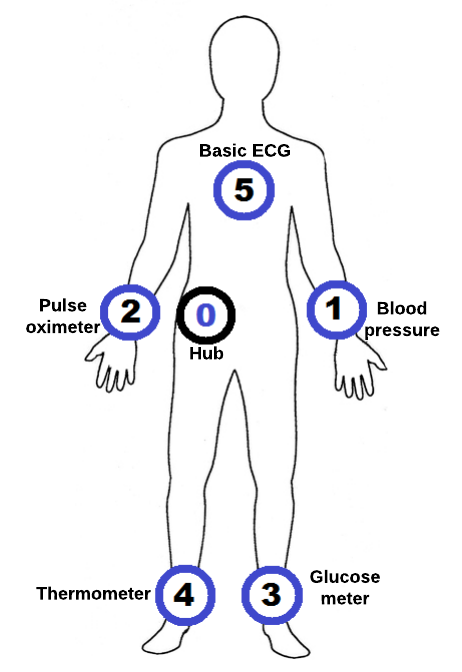
\includegraphics[scale=0.29]{figures/corpoSensoresNomes.png}}
\caption{The simulated network topology.}
\label{fig:wbantopology}
\end{figure}

In this work we simulate six scenarios, three agent-initiated and three manager-initiated.

The first three agent-initiated scenario are: a) Unconfirmed Mode, where the agents takes the initiative to send measurements to the manager without confirmation. b) Confirmed Mode, agents wait for three seconds the ACK from the manager. If an ACK is not received, the agent has to try to establish a new association to finalize the transmission of the measurement packets. c) Retransmission Mode, agents expect an ACK from the manager during the time period defined by the user in \textit{timeOutToRetransmitPacke} and in case it is not received, the packet is retransmitted up to \textit{maxNumOfRetransmition} also define by the user. If all the retries is used and an confirmation is not received, a new association is made. 

The last three manager-initiated scenarios are: a) Single Mode, the manager request just one measurement data to an agent. b) Time Period mode, allows manager to request agents to send measurements data during a time period. c) and finally, the No Time Period Mode where manager request measurements data to the agents continually until the association is break or the manager sends a \textit{Stop Request} message.
%Table \ref{3modes} summarizes the three mentioned modes. 

The MAC layer used is the IEEE 802.15.6 (WBAN) \cite{b5} with path loss map and temporal model for wireless channel supplied by Castalia. The radio used meets with the IEEE 802.15.6 radio proposal \cite{b5} with $-15$dBm as transmission power.
% \begin{table}[htbp]
% \caption{Operational modes supported by the proposed implementation}
% \begin{center}
% \begin{tabular}{lllll}
% \cline{2-4}
%  & \multicolumn{1}{c}{\textbf{\begin{tabular}[c]{@{}c@{}}Unconfirmed\\ mode\end{tabular}}}                      & \multicolumn{1}{c}{\textbf{\begin{tabular}[c]{@{}c@{}}Retransmission\\ mode\end{tabular}}}                                      & \multicolumn{1}{c}{\textbf{\begin{tabular}[c]{@{}c@{}}Confirmed\\ mode\end{tabular}}}                                         &  \\ \cline{2-4}
%  & \begin{tabular}[c]{@{}l@{}}The measurements \\ are transmitted\\ with no ACK from\\ the manager\end{tabular} & \begin{tabular}[c]{@{}l@{}}The measurements \\ are retransmitted\\ if an ACK is not\\ received from the\\  manager\end{tabular} & \begin{tabular}[c]{@{}l@{}}If an ACK is not\\ received, try a\\ new association\\ to continue the \\ transmission\end{tabular} &  \\ \cline{2-4}
% \end{tabular}
% \label{3modes}
% \end{center}
% \end{table}

The configuration of the nodes is set as follows: the total simulation time is $43200$ seconds (12 hours). Node 0 uses the \textit{Manager} application and is the hub. The blood pressure monitor transmits one measurement every $15$ minutes, totalizing $48$ measurements to be sent in our simulation. The thermometer sends one read every $3$ minutes, then, $240$ measurements should be sent. The glucose meter transmits one measurement every $5$ minutes, that is, $144$ measurements in  $43200$ seconds. Thermometer sends the temperature every $3$ minutes then $240$ in total. In this work, we assume the basic ECG as a device that receives signals of all electrodes deployed in the body, and transmit these signals to the manager. So, it will transmit $80$ millivolt samples per $0.8$ seconds, which gives $54000$ measurement packets in $43200$s of simulation.

In the three agent-initiated modes the nodes will try to transmit all the packets described in the paragraph above, but in manager-initiated modes it is not true. The Single Mode for example, transmit just one measurement data packet. For the Time Period Mode we define $21600$ seconds ($6$ hours) of measurement data packets transmission, which is half of the total measurements transmitted in agent-initiated modes. And for the No Time Period mode the manager sends a \textit{Stop Request} message when $10$ measurement data packet is received from every node.     

\section{Results}\label{results}

%All the results that will be presented is already implemented in the proposed application and everyone can feel free to customize it. 
%The results available in the application are the total control packets exchanged per node, the measurements packets received by the manager per node, the measurements packets sent by each node, and the total of associations made per agent. 

The first result discussed is the total of successfully measurements delivered to the manager using the agent-initiated mode.
%As described in \cite{b1}, when an agent is working on confirmed mode, it  should send a measurement packet and wait for the ACK during three seconds.
We can see in Figure~\ref{fig:measurementsDeliveredAgentInitiated} the delivered packets from ECG using confirmed mode is too small. This shows the lack of adaptation of the confirmed mode when the interval to transmit the measurements packet is smaller than the timeouts proposed by the standard. In this case, the bad link quality and consequently the loss of ACKs, use of timeouts for disassociation/reassociation processes took most of the time for measurement transmission. For example, in our simulation the ECG sends one measurements every 0.8s, a timeout for the association process in confirmed mode takes 10s, that is, 12.5 packets that could be transmitted in this timeout period.
The retransmission mode improved the results by reducing the wait time of an association handshake, and retransmitting the messages sooner. The unconfirmed mode delivered almost all packets, although it provides no reliability.
In contrast to the ECG, the thermometer in confirmed mode, Figure~\ref{fig:measurementsDeliveredAgentInitiated}, delivered more than 100\% of the measurement packets because duplicate measurements are taken into account for this result.

\begin{figure}[htbp]
\centerline{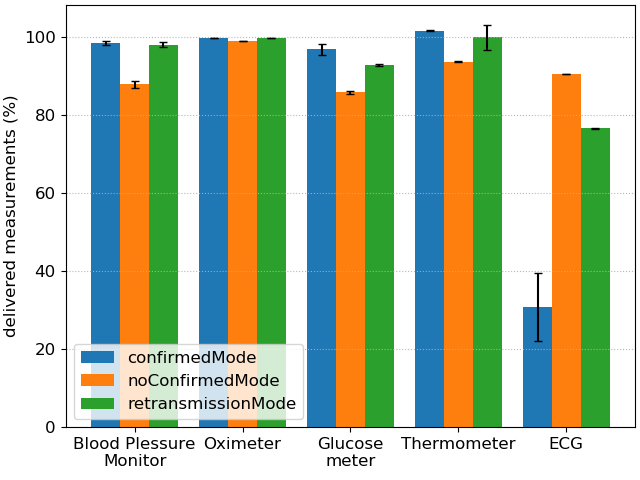
\includegraphics[width=\linewidth]{figures/MeasurementsDelivered-AgentinitiatedMode.png}}
\caption{Measurement packets successfully delivered per node using Agent-initiated mode}
\label{fig:measurementsDeliveredAgentInitiated}
\end{figure}

The delivered measurements packets for the manager-initiated mode can be seen in the Figure~\ref{fig:measurementsDeliveredManagerInitiated}.

\begin{figure}[htbp]
\centerline{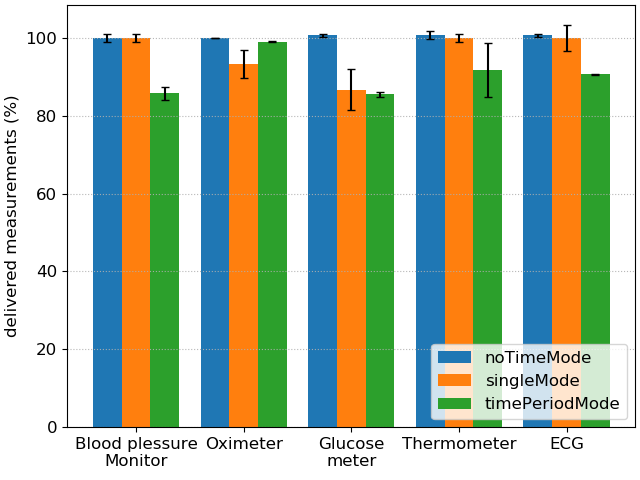
\includegraphics[width=\linewidth]{figures/MeasurementsDelivered-ManagerinitiatedMode.png}}
\caption{Measurement packets successfully delivered per node using Manager-initiated mode}
\label{fig:measurementsDeliveredManagerInitiated}
\end{figure}

The overhead of control packets exchanged between a node and the manager is crucial in this scenario, as in the case of a new association due to a non-received ACK. The association procedure involves a maximum of four packets for a new node, and a minimum of two packets, when the agent's attributes are previously known.

The total of control packets exchanged between each node and the manager per operation mode is depicted in Figure~\ref{fig:controlpacketsexchanged}.
Notice that nodes transmit different number of packets in the same simulation. While the blood pressure monitor convey $48$ measurements in $12$ hours, the ECG has to transmit $54000$ measurements in the same time period. Is expected to save more control packets in retransmission mode when compared to confirmed mode. Although, the ECG in Figure~\ref{fig:controlpacketsexchanged}, the retransmission mode has used more control packets than the confirmed mode due to the first one delivered more measurements packets than the former mode as was seen in Figure~\ref{fig:measurementsDeliveredAgentInitiated}.
%Notice that our retransmission mode saves about $21.5\%$ of control packets when compared to the confirmed mode. 
The unconfirmed mode as expected is the one that transmits less control packets.

\begin{figure}[htbp]
\centerline{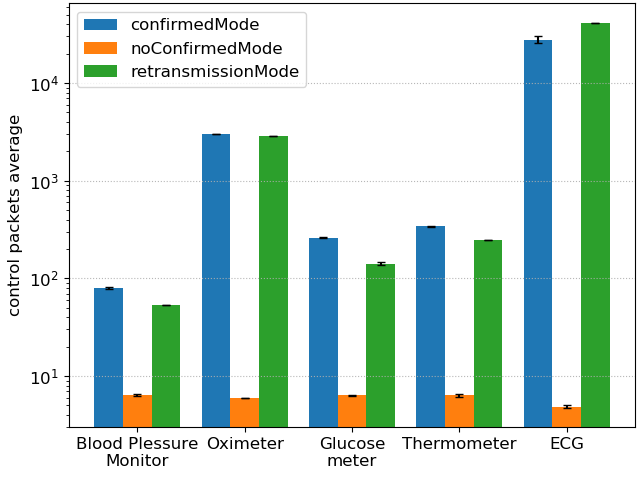
\includegraphics[width=\linewidth]{figures/ControlPacketsPerNode.png}}
\caption{The average control packets exchanged of all nodes in Agent-initiated mode.}
\label{fig:controlpacketsexchanged}
\end{figure}

The number of associations made per node is extremely high with the confirmed mode, since it tries a new association after every packet lost. Figure~\ref{fig:associationnumber} shows the average number of associations that each node made in Agent-initiated modes. As expected, the confirmed mode has the highest average of association attempts, while the unconfirmed mode made just one association. The retransmission mode tries a new association after all the attempts to resend a message, or if the agent receives an abort message from the manager. This is the reason for the low average of associations in this mode. The ECG which has the worst wireless link require almost $2000$ new associations to finalize the transmission of $54000$ measurements in confirmed mode.

\begin{figure}[htbp]
\centerline{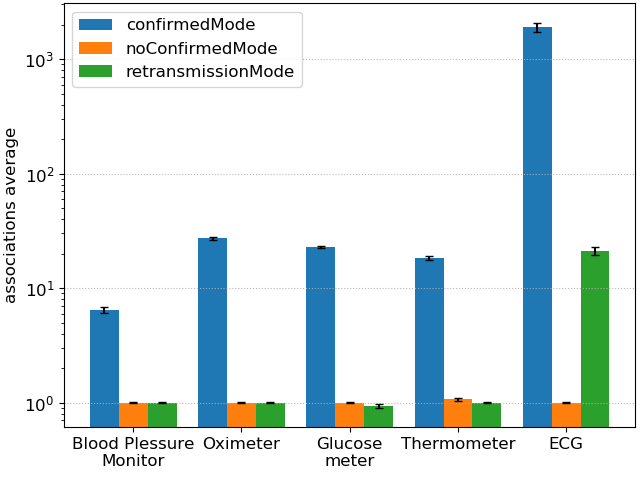
\includegraphics[width=\linewidth]{figures/AssociationsMadePerNode.png}}
\caption{The average numbers of association made per node}
\label{fig:associationnumber}
\end{figure}

In the Figure~\ref{fig:retransmissionretries} we can see the average number of retransmission retries made in the retransmission mode by the application layer. Most packets are successfully delivered in the first try and more than $1000$ packets uses $1$ retransmission retry. In the seventh retransmission retry the values tend to zero.

\begin{figure}[htbp]
\centerline{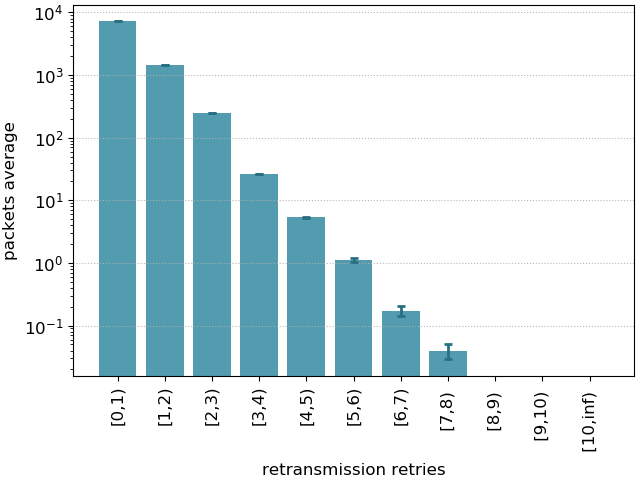
\includegraphics[width=\linewidth]{figures/RetransmissionRetries.png}}
\caption{The average number of packets retransmission made at the application layer}
\label{fig:retransmissionretries}
\end{figure}

The Figure~\ref{fig:latency} shows that most packages have an average latency of $180$ms in retransmission mode and confirmed mode and $30$ms in no confirmed mode. 
The time is calculated from the moment of creation of the package, at the application layer of the agent, until it is received at the application layer of the manager.

\begin{figure*}[htbp]
\centerline{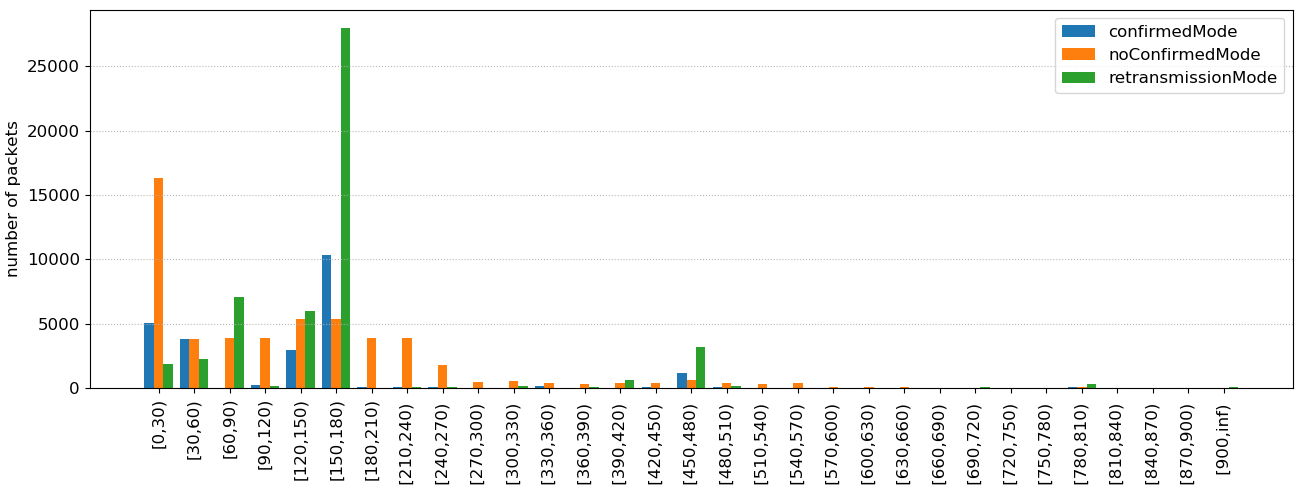
\includegraphics[width=\linewidth]{figures/Latency.png}}
\caption{The latency level in application layer}
\label{fig:latency}
\end{figure*}